\chapter{Time metrology}
Aim of this chapter is to present an issue that will be dealt with in this work.
First a concept of theoretical clock will be presented alongside mathematical tools required
for it description and behavior modelling.
This is followed by a more detailed description of stability analysis which is most prominent
field of science dealing with clock behavior.
After describing theoretical clock models an attention will be given to physical implementation
of clock system with special focus on types of clocks used aboard GPS satellites.
Finally current state of the art in GPS clock bias prediction will be presented.
Intention of writing this chapter was that despite clock modelling and frequency analysis being
well known field readers with computer science might not be familiar with it.
For those well versed in frequency analysis most of this chapter can be safely skipped with 
exception of last section that focuses on state of the art in GPS clock prediction as it 
deals with issues that are more specific do described in this work.
It is important to understand that this chapter do not provide comprehensive knowledge about
described field as due to methodology used in presented work that knowledge it is not required.
For more information about clock modelling and stability analysis Handbook of Frequency Stability
Analysis is suggested as reading.



%====================================================================================================
\section{Mathematical clock model}
In context of pure mathematical modelling a clock is understood as a function that describes
offset between two given values for a specific point in time. One of those values is referred 
to as the reference clock and it is considered to always return correct time $T_{r}(t)=t$.
It is important to understand that in physical systems value of $t$ is not only inaccessible, as
every measurement instrument have some degree of uncertainty, but do not exists at all.
This is due to time dilatation effect, derived from special theory of relativity, that causes
time to flow differently in systems that move with velocities close to speed of the light.
This issue is dealt with by selecting most precise physical clock available as the reference
clock and modelling difference between it and other clocks, including time dilatation effects,
as their bias.
Main goal of modeling clocks is to retrieve a value of $t$, which is equal to $T_{r}(t)$, based
on value read from given clock $T_{c}(t)$. 
As relation between those clock is fully described by analyzed clock bias 
$b_{c}(t)=T_{r}(t)-T_{c}(t)$ clock model is equivalent to just a bias model.

%----------------------------------------------------------------------------------------------------
\subsection{Discrete and continuous clock models}
There are two possible approaches to mathematical clock modelling, one of them is continuous
clock model that relies on differential equation for description of its behavior.
In this approach clock bias is modeled as :
\begin{equation}
	\label{equ:continous_clock}
	b_{c}(t) = T_{r}(t_{0}) +  \int_{t_{0}}^{t} \varepsilon_{c}(\tau) d\tau ,
\end{equation}
where:
\begin{itemize}
	\item $t$ is the independent time argument,
	\item $b_{c}(t)$ is the clock bias at time $t$,
	\item $t_{0}$ is time at which clock was synchronized with reference ($b_{c}(t_{0})=0$),
	\item $T_{r}(t_{0})$ is value of reference clock at $t_{0}$,
	\item $\varepsilon_{c}(\tau)$ is the normalized frequency offset of a clock.
\end{itemize}
The branch of science that deals with continuous clock modelling is called stability analysis.
In this work no more attention will be given to that approach as due to nature of data as well as
choice of prediction algorithms favour a discrete clock model.
In discrete clock model bias is described as :
\begin{equation}
	\label{equ:discrete_clock}
	b_{c}(i) = T_{r}(i) - T_{c}(i),
\end{equation}
where $i \in \mathbb{N}$ is the number of measurement.
One of main differences between continuous and discrete models is that in latter case bias is 
considered only as a difference between two individual measurements where in case of 
continuous model all differences starting from synchronization are taken into account.
Another important change is that in discrete model clock is a function $\mathbb{N} \to \mathbb{R}$
instead of $\mathbb{R} \to \mathbb{R}$ like it was in case of continuous model. 
This requires redefinition of reference clock from $T_r{t}=t$ into:
\begin{equation}
	\label{equ:discrete_reference}
	T_{r}(i) = \Delta T_r i,
\end{equation}
where $\Delta T_r$ is the measurement period of reference clock.
In such model $T_{r}$ as well as $T_{c}$ are time series which means that $b_{c}$ is also one.
This means that methodologies related to time series analysis like \textbf{TODO : LIST METHODS}
can be used.
Usually clocks are modelled as a linear combination of several deterministic and stochastic 
components as shown on Figure \ref{fig:clocks_example}. 
\begin{figure}[htb] 
\label{fig:clocks_example}
\centering
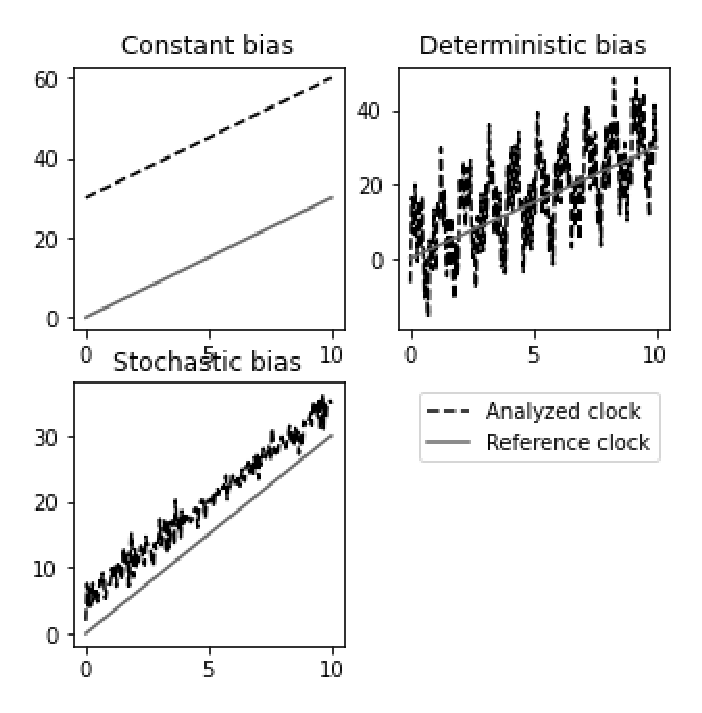
\includegraphics[width=\textwidth]{figures/bias_examples}
\caption{Example of clock readouts depending of nature of their bias}
\end{figure}
More information on exact clock and noise models will be given in following sections.

%----------------------------------------------------------------------------------------------------
\subsection{Basic clock model}

%----------------------------------------------------------------------------------------------------
\subsection{Modeling noise}

%----------------------------------------------------------------------------------------------------
\subsection{Standard clock model}




%====================================================================================================
\section{Physical clock implementation}

%----------------------------------------------------------------------------------------------------
\subsection{Introduction to physical clock implementation}

%----------------------------------------------------------------------------------------------------
\subsection{Principles of atomic clock design}

%----------------------------------------------------------------------------------------------------
\subsection{Time measurement on orbit}


%====================================================================================================
\section{State of the art in GPS clock bias prediction}

%----------------------------------------------------------------------------------------------------
\subsection{Time references in GPS}

%----------------------------------------------------------------------------------------------------
\subsection{Satellite broadcast polynomial}

%----------------------------------------------------------------------------------------------------
\subsection{IGU products}
